In order to test whether the motors of the robot could move in a synchronised
way, using the protocol described in \autoref{ssec:motortest}, we developed a
Python script (using the OpenCV\footnote{\url{http://opencv.org/}} library) that could analyse a video of the
wheels spinning and measure the rotation periods.

\beforelist* The analysis is done on a series of frames (extracted from a video
by using FFmpeg\footnote{\url{https://ffmpeg.org/}}) with the assumptions that:
\begin{enumerate}
  \item the wheel axis is almost aligned with the camera;
  \item two markers of the same color contrasting with the surrounding are
    placed on the wheel, one on the axis and one on the circumference.
\end{enumerate}
\afterlist*
The script tracks these two markers to esteem the orientation of the wheel in
each frame, using this information to measure the rotation speed.
From now on, the two markers will be called \emph{axis} and \emph{marker} to
distinguish them.

\beforelist* There are various configuration options that must be set before
starting the analysis to get an accurate result (most of them are represented
in \autoref{fig:motconf}):
\begin{description}
  \item[Cropping area:] only this area of the image is used for the analysis,
    everything else is ignored;
  \item[Starting axis coordinates:] it indicates where in the image the axis
    is approximately located (during the analysis the axis position is
    continually updated using the last match to account for slight movements of
    the camera or the wheel);
  \item[Maximum axis movement:] this is the maximum distance that a detected
    point can be from the old axis position to be considered a good candidate
    for the new axis position;
  \item[Minimum marker distance:] this is the minimum distance that a detected
    point has to be from the old axis position to be considered a good candidate
    for the new marker position;
  \item[Approximate marker distance:] it esteems the distance of the marker from
    the axis (length that should remain roughly constant), creating a
    circumference where the marker is expected to be;
  \item[Marker predominant channel:] it defines whether the color of the marker
    should be considered blue, green or red during the analysis;
  \item[Marker threshold:] this is the value used to decide whether a pixel of
    the image is probably part of a marker or not (in the following description
    of the various steps this will become clearer);
  \item[Approximate marker size:] it indicates how many grouped pixels must be
    detected \emph{at least} to consider the group a probable marker;
  \item[Pass angle:] this is the angle from the horizontal used to count the
    rotations and defines the \emph{pass line}. 
\end{description}
\afterlist*

\begin{figure}
\begin{subfigure}[t]{0.5\textwidth}
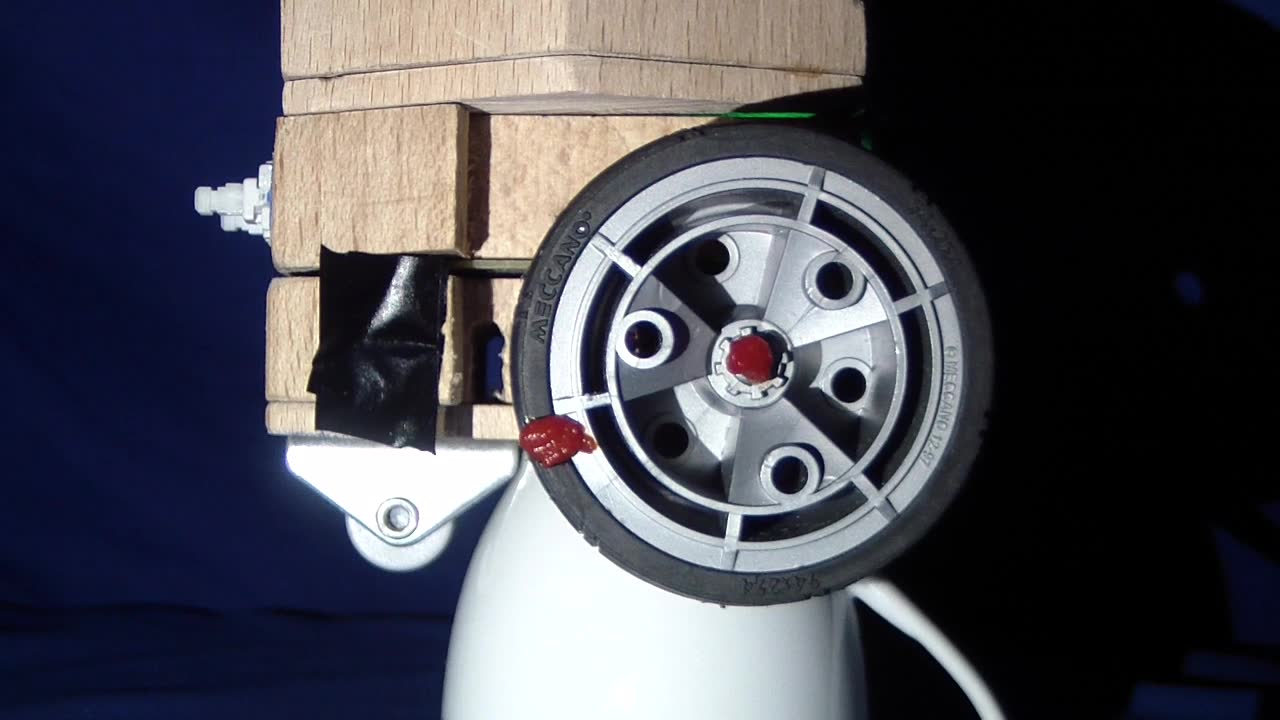
\includegraphics[width=\textwidth]{img/motan_base}
\caption{Original image}
\label{fig:motbase}
\end{subfigure}
\begin{subfigure}[t]{0.5\textwidth}
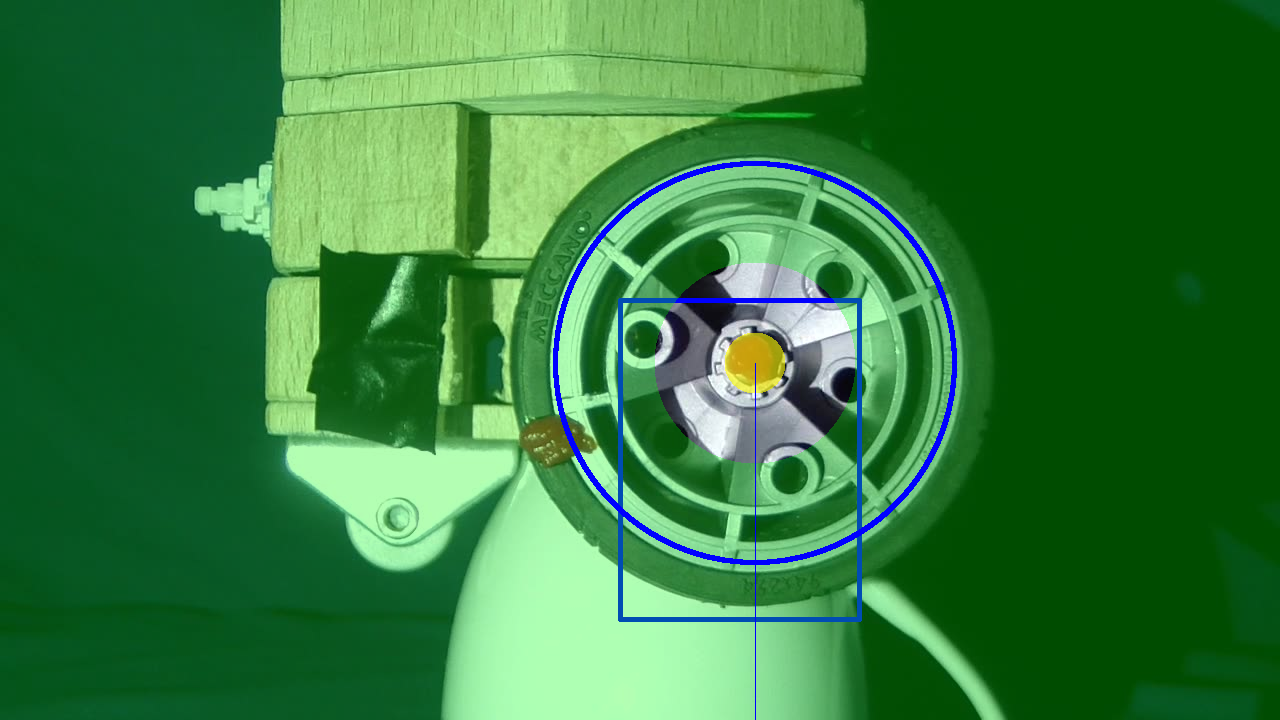
\includegraphics[width=\textwidth]{img/motan_conf}
\caption{Image with configuration options overlayed}
\label{fig:motoverlay}
\end{subfigure}
\caption[Graphical representation of the configuration options]{
  Graphical representation of the configuration options

  The blue rectangle indicates the cropping area, the blue circle defines the
  expected path of the marker, the thin blue line corresponds to the
  \emph{pass line}, the yellow and green areas are respectively where the axis
  and the marker can be located.
  }
\label{fig:motconf}
\end{figure}

\beforelist* During the analysis, the following steps are carried out for each
frame to measure the current orientation of the wheel (they are shown in
\autoref{fig:motstep}):
\begin{enumerate}[label=\alph*)]
  \item the frame is cropped to the cropping area and framed with a black border
    (to avoid problems with OpenCV's blob detection);
  \item a greyscale value is calculated for each pixel, using the formula
    \[
      value = 255\cdot\frac{c}{r + g + b}
    \]
    \begin{tabbing}
      where:  \= $value$ is the greyscale value \\
              \> $c$ is the value of the pixel corresponding to the marker
                channel \\
              \> $r$ is the red channel value of the pixel \\
              \> $g$ is the green channel value of the pixel \\
              \> $b$ is the blue channel value of the pixel
    \end{tabbing}
  \item a threshold is applied to the filtered frame to extract blocks of pixels
    which color is mostly that of the marker channel;
  \item the OpenCV \Code|SimpleBlobDetector| is used to detect and locate blocks
    of continous black pixels (considering the minimum size defined by the
    configuration options), from which the best matches are extracted.
\end{enumerate}
\afterlist*

\begin{figure}
\begin{subfigure}{0.25\textwidth}
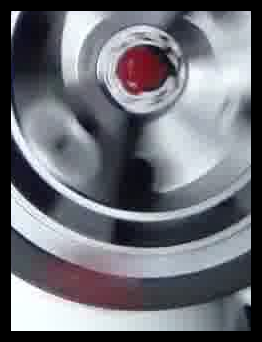
\includegraphics[width=\textwidth]{img/motan_1}
\caption{Crop}
\label{fig:motcrop}
\end{subfigure}%
\begin{subfigure}{0.25\textwidth}
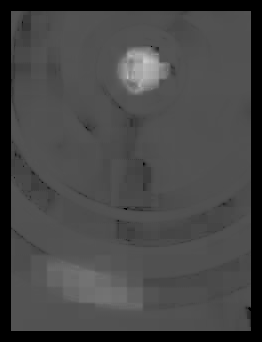
\includegraphics[width=\textwidth]{img/motan_2}
\caption{Filter}
\label{fig:motred}
\end{subfigure}%
\begin{subfigure}{0.25\textwidth}
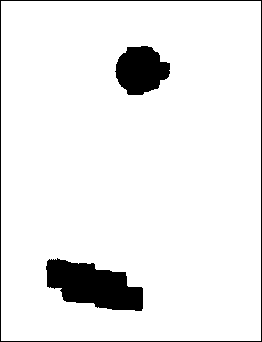
\includegraphics[width=\textwidth]{img/motan_3}
\caption{Threshold}
\label{fig:motblob}
\end{subfigure}%
\begin{subfigure}{0.25\textwidth}
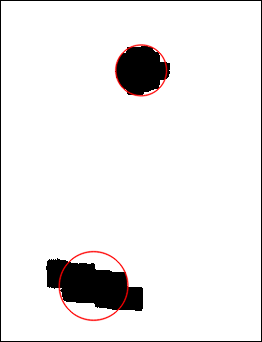
\includegraphics[width=\textwidth]{img/motan_4}
\caption{Blob detection}
\label{fig:motkey}
\end{subfigure}
\caption{Steps of the analysis of a frame}
\label{fig:motstep}
\end{figure}

\beforelist* The best matches are decided according to the rules defined by the configuration options, that is:
\begin{itemize}
  \item the detected axis position can't be too far from the old axis position;
  \item the detected marker position can't be too near to the detected axis
    position;
  \item if more than one axis candidate is detected, the one nearest to the old
    axis position is chosen (its position becomes the axis position for the next
    frame);
  \item if more than one marker candidate is detected, the one which distance
    from the axis is closer to the \emph{approximate marker distance} is used.
\end{itemize}
\afterlist*
If both the axis and the marker were succesfully detected, the angle of rotation
is estimated from their position:
\[
  \theta = \mathrm{atan2}\left( M_y-A_y, M_x-A_x \right) - \theta_0
\]
\begin{tabbing}
where:  \= $\theta$ is the angle of rotation \\
        \> $A_x$ is the $x$ position of the axis \\
        \> $A_y$ is the $y$ position of the axis \\
        \> $M_x$ is the $x$ position of the marker \\
        \> $M_y$ is the $y$ position of the marker \\
        \> $\theta_0$ is the pass angle
\end{tabbing}

When, between two frames, the angle changes sign, a new rotation is counted.
The time of crossing is then calculated by assuming a constant angular speed
between the two frames:
\[
  time = \frac{1}{FPS}\left( \#frame - \frac{\theta}{\theta - \theta_p} \right)
\]
\begin{tabbing}
where:  \= $time$ is the time of crossing \\
        \> $FPS$ is the framerate of the original video \\
        \> $\#frame$ is the index of the current frame \\
        \> $\theta$ is the angle of rotation in the current frame \\
        \> $\theta_0$ is the angle of rotation in the previous frame 
\end{tabbing}
By subtracting the time of consecutive crossings, the rotation periods are
computed.

\textit{Important note: since this algorithm hasn't been properly validated yet,
it is not suggested to trust its results without questions. It should only be
used to speed up measures and calculations while supervising it to check if the
correct passing frames are detected.}
